\section{Diseño de la red y Routemap en Packet Tracer}

El diseño de la red constituye una etapa fundamental dentro del desarrollo del proyecto, ya que permite establecer la base lógica y física sobre la cual se implementan los servicios de red y se ejecutan las actividades de seguridad informática. En este apartado se describe de manera detallada la topología propuesta por el Grupo 6, así como la interconexión de los dispositivos y el flujo de comunicación entre las diferentes redes.

La topología fue diseñada y simulada utilizando la herramienta \textbf{Cisco Packet Tracer}, lo que permitió validar previamente la conectividad, la segmentación de la red y el correcto funcionamiento del enrutamiento inter-VLAN antes de proceder con las configuraciones finales.

\subsection{Descripción general de la topología}

La red diseñada está compuesta por un \textbf{router Cisco 2811}, un \textbf{switch Cisco 2960-24TT}, un \textbf{Access Point}, y cuatro equipos finales distribuidos en tres redes lógicas independientes. La interconexión de estos dispositivos permite simular un entorno realista en el que coexisten redes cableadas e inalámbricas, así como estaciones de trabajo y servidores.

El switch actúa como el punto central de distribución del tráfico, conectando tanto al router como a los equipos finales y al Access Point. El router, por su parte, se encarga del enrutamiento entre las distintas VLANs configuradas, permitiendo la comunicación controlada entre las redes.

\subsection{Segmentación de la red}

La infraestructura fue segmentada en múltiples redes lógicas mediante el uso de \textbf{VLANs}, lo que permite aislar el tráfico de cada red, mejorar el rendimiento general y aumentar el nivel de seguridad. Cada VLAN corresponde a una red específica definida en el enunciado del proyecto:

\begin{itemize}
    \item \textbf{Red X1}: Red destinada a pruebas de seguridad, integrada por el sistema Kali Linux y el Access Point.
    \item \textbf{Red X2}: Red de servidores, representada por un equipo con Windows Server.
    \item \textbf{Red X3}: Red de usuario final, correspondiente al equipo PCGX.
\end{itemize}

Adicionalmente, se configuró una VLAN adicional destinada a pruebas y validaciones internas, lo que permitió realizar configuraciones y comprobaciones sin afectar el funcionamiento de las redes principales.

\subsection{Esquema de direccionamiento IP}

El direccionamiento IP utilizado en la práctica se basa en el rango de direcciones privadas \texttt{192.168.X.0/24}, donde el valor \textbf{X} corresponde al número del grupo, en este caso el Grupo 6. De esta manera, las redes quedan estructuradas de la siguiente forma:

\begin{itemize}
    \item VLAN 10 – Red Kali Linux y Access Point: \texttt{192.168.61.0/24}
    \item VLAN 20 – Red Windows Server: \texttt{192.168.62.0/24}
    \item VLAN 30 – Red PCGX: \texttt{192.168.63.0/24}
    \item VLAN 40 – Red de pruebas: \texttt{192.168.64.0/24}
\end{itemize}

Cada red cuenta con su respectiva puerta de enlace predeterminada configurada en el router, garantizando la correcta comunicación entre VLANs mediante enrutamiento inter-VLAN.

\subsection{Enrutamiento inter-VLAN}

Para permitir la comunicación entre las distintas redes, se implementó un esquema de \textbf{Router-on-a-Stick}, utilizando subinterfaces en la interfaz física del router conectada al switch. Cada subinterface fue configurada con encapsulación \textbf{IEEE 802.1Q}, asociándola a una VLAN específica y asignándole la dirección IP correspondiente.

Este enfoque permite optimizar el uso de interfaces físicas del router y facilita la administración del enrutamiento, manteniendo una estructura clara y organizada.

\subsection{Flujo de comunicación de la red}

El flujo de datos dentro de la red se desarrolla de la siguiente manera:

\begin{enumerate}
    \item Los equipos finales envían el tráfico hacia su puerta de enlace predeterminada, correspondiente a la subinterface del router asociada a su VLAN.
    \item El switch identifica la VLAN de origen y transporta el tráfico etiquetado a través del enlace troncal hacia el router.
    \item El router procesa el tráfico y determina la red de destino, reenviando los paquetes hacia la VLAN correspondiente.
    \item El switch distribuye el tráfico hacia el puerto de acceso donde se encuentra conectado el dispositivo de destino.
\end{enumerate}

Este flujo garantiza que la comunicación entre redes se realice de manera controlada, permitiendo además aplicar políticas de seguridad y monitoreo sobre el tráfico inter-VLAN.

\subsection{Diagrama de la topología}

En la Figura \ref{fig:topologia} se presenta el diagrama de la red diseñado en Cisco Packet Tracer, donde se puede observar la interconexión entre el router, el switch, el Access Point y los equipos finales, así como la segmentación lógica implementada mediante VLANs.

\begin{figure}[H]
    \centering
    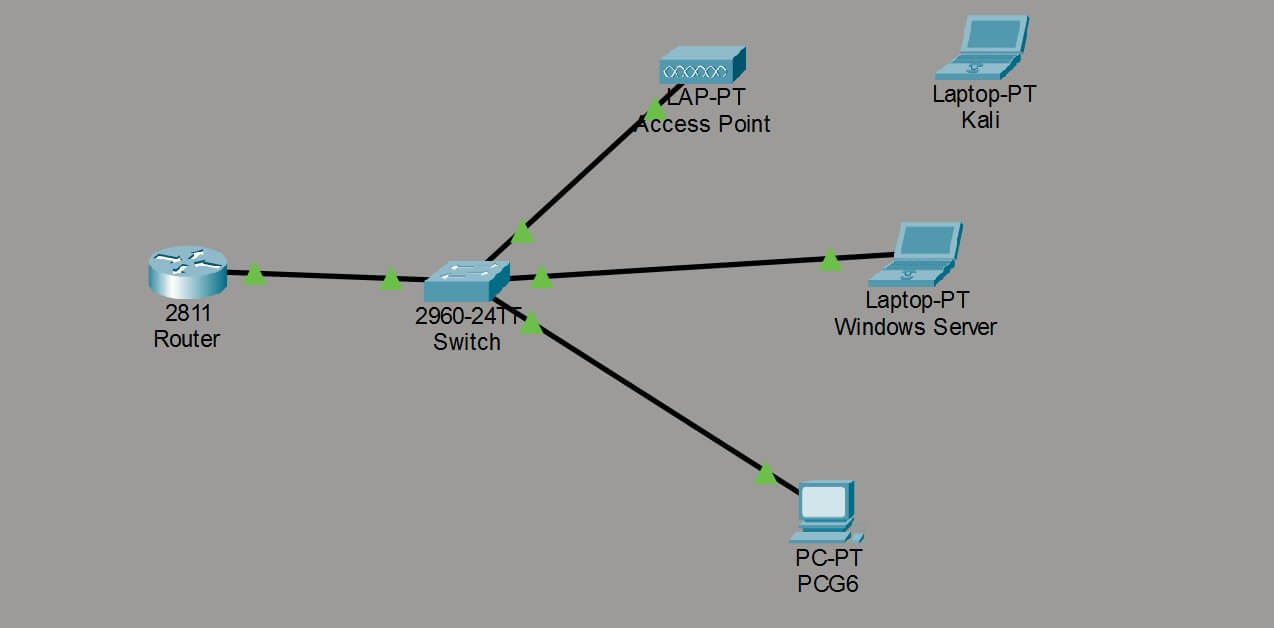
\includegraphics[width=0.9\textwidth]{assets/images/topologia_packet_tracer.jpeg}
    \caption{Topología de red diseñada en Cisco Packet Tracer}
    \label{fig:topologia}
\end{figure}

La topología diseñada permite cumplir con los requisitos establecidos en el enunciado del proyecto, proporcionando una infraestructura adecuada para la ejecución de las actividades de seguridad informática documentadas en los capítulos posteriores.
